\documentclass[main.tex]{subfiles}
\begin{document}

\chapter{Introduction}

I hope readers will find this article useful, but at the outset I say this: I am writing for myself. As I get older, I find it easier to learn things by summarizing them as though I were to teach them. Feedback is appreciated, but don't expect a fully-formed set of lessons. Not yet, anyway. I am at the beginning of this path.
(Also, I'm sorry that I switch around transliterations and scripts, I learned Cyrillic and still haven't learned the new Latin script.)

Basically every textbook begins with the following basic information, so I will too:
\begin{itemize}
	\item Qazaq is a \textbf{Turkic} language with a (generally) \href{https://en.wikipedia.org/wiki/Subject-object-verb_word_order}{SOV}, \href{https://en.wikipedia.org/wiki/Head-directionality_parameter}{head-final} grammar.(Similar to Japanese, Korean, etc. Also similar to Japanese, this word order can be departed from for poetic effect. )
	
	\item It is a \href{https://en.wikipedia.org/wiki/Synthetic_language}{\textbf{synthetic}} language. (Words are altered, or "inflected" to show the roles that they take on in a sentence. This is like Latin or Japanese, and unlike English, which is an analytic language.)
	
	\item It is an \href{https://en.wikipedia.org/wiki/Agglutinative_language}{\textbf{agglutinative}} language. (A series of affixes is added to the stem of a word to alter its meaning. This is again similar to Japanese.)
\end{itemize}

\section{Agglutination}
In order to build a meaning from a root word, Qazaq adds affixes (Аффикс) to the word, altering its meaning. An example from English would be book+s = books.
Inflected forms may become quite complicated, with many affixes. Famously, one of the longest words in Qazaq is:

қанағаттандырылмағандықтарыңыздан

қанағат-тан-дыр-ыл-ма-ған-дық-тарыңыз-дан (\href{https://www.quora.com/What-is-the-longest-word-in-Kazakh}{Thanks to "Muhamed Ali Ospan" on Quora.})\\
Which I believe means "As a result of your (plural) having been caused dissatisfaction".

To form sentences of any degree of complexity, we will need to learn this system. It will take several lessons.

(In a few cases, Qazaq also uses prefixes, but they are few and will be handled later.)


%%
%%
%%
\section{Vowel Harmon and Consonant Assimilation}
%%TODO
\todo{Rewrite this all to sound better.}{}
Again the first lesson in most textbooks is about vowel harmony and consonant assimilation. These are rules where the type of sounds that appear in a word dictate which type of sounds come in the affixes added later during inflection.
%%%[TODO: I will try to expand this in the future.]

\begin{itemize}
	\item \textbf{Vowel harmony} refers to preferring the same kinds of vowels throughout the final inflected form. It can also have an effect on the choice of consonant.
	\item \textbf{Consonant assimilation} is the system by which the consonants of each ending are chosen based on previous sounds.
\end{itemize}
%%%[TODO: Add detailed explanations and pictures/state-transition-diagrams for both]

%%% VOWEL HARMONY %%%%
\subsection{Vowel Harmony}
\href{https://en.wikipedia.org/wiki/Vowel_harmony#Kazakh}{Vowel Harmony} (\href{https://kk.wikipedia.org/wiki/\%D0\%94\%D0\%B0\%D1\%83\%D1\%8B\%D1\%81\%D1\%82\%D1\%8B\%D0\%BB\%D0\%B0\%D1\%80_\%D2\%AF\%D0\%BD\%D0\%B4\%D0\%B5\%D1\%81\%D1\%82\%D1\%96\%D0\%B3\%D1\%96}{Дауыстылар үндестігі}) is the process by which vowels in a word must be of the same kind.

Vowels are divided into categories over three dimensions (front/back, round/unround, closed/open). For now, the most important dimension is front/back:

\begin{itemize}
	\item \textbf{Back} (жуан): а ы о ұ э у
	\item \textbf{Front} (жіңішке): ә е і ө ү и
\end{itemize}

( \href{https://www.youtube.com/watch?v=f7ci3zddACg}{See this video for example pronunciations.} \href{https://www.youtube.com/watch?v=Ht5XWZe8SSY}{This one.} \href{https://www.youtube.com/watch?v=SRi_7zrZjyA\&t=96s}{Also this one.} )

\begin{figure}[H]
	\centering
	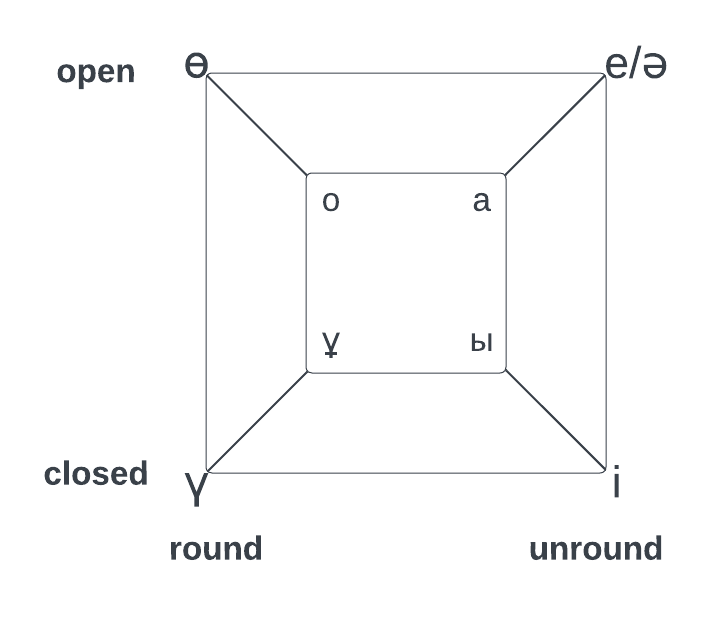
\includegraphics[width=0.75\textwidth]{kk-vowels-3d.png}
	\caption{Most of the vowels of Qazaq, presented in three dimensions}
\end{figure}

A (native) word may only contain all front or all back vowels. When appending affixes, you will have a choice of several equivalent suffixes (called \href{https://en.wikipedia.org/wiki/Morpheme#Allomorphs}{allomorphs}), and must choose the one that harmonizes with the word so far. (For loanwords, harmonize with the final vowel.)

For example, the plural endings are \textbf{лар/лер}, \textbf{дар/дер}, \textbf{тар/тер}. You choose one of the three pairs according to the correct consonant (discussed next), and within that pair, the one which harmonizes the vowels.

\subsubsection*{Examples for Vowel Harmony}
To pluralize \textbf{бала} (child), you choose \textbf{лар/лер} and find the one using a back vowel:  \textbf{бала + лар} : \textbf{балалар} (children).

\textbf{Мұғалім} (teacher) becomes \textbf{мұғалім+дер}. Notice that this Arabic-derived loanword (through Persian) does not internally follow vowel harmony, but we use the last vowel in the word to guide our choice for additional affixes.

%%% CONSONANT ASSIMILATION %%%%
\subsection{Consonant Assimilation}
\href{https://en.wikipedia.org/wiki/Consonant_harmony}{Consonant assimilation} (\href{https://kk.wikipedia.org/wiki/\%D0\%94\%D0\%B0\%D1\%83\%D1\%8B\%D1\%81\%D1\%81\%D1\%8B\%D0\%B7\%D0\%B4\%D0\%B0\%D1\%80_\%D2\%AF\%D0\%BD\%D0\%B4\%D0\%B5\%D1\%81\%D1\%82\%D1\%96\%D0\%B3\%D1\%96}{Дауыссыздар үндестігі}) is a process whereby consonants earlier in the word dictate consonants that come later in the word.

Historically, the consonants of Qazaq are divided into three categories by the degree of their sonority  \href{https://oozcelik.pages.iu.edu/papers/Kazakh\%20phonology.pdf}{[link]} \href{https://itest.kz/kz/ent/qazaq-tili/fonetika/lecture/dauyssyz-dybystar-qatang-uyang-undi-dauyssyzdar-emlesi}{[link]}. For our needs, we will further subdivide these categories:
\begin{itemize}
	\item (Vowels are the most sonorous, before consonants.)
	\item Sonorants (Үнді): й у р / л / м н ң
	\item Voiced (Ұяң): в ж з / б д г ғ
	\item Unvoiced (Қатаң): һ с ф х ц ч ш щ / п т к қ [TODO: This list isn't yet fully sorted. Subject to minor revisions.]
\end{itemize}

\subsubsection{Progressive Consonant Assimilation}
Generally, the last sound in a word so-far will predict that the next affix starts with a consonant of equal or lesser sonority.

Examples for Progressive Consonant Assimilation using plurals:
\begin{itemize}
\item Бала. Бала+лар. (Vowel -> Sonorant)
\itemАға. Аға+лар. (Vowel -> Sonorant)
\\
\itemҚой. Қой+лар. ((high) Sonorant -> (medium) Sonorant)
\itemСу. Су+лар. ((high) Sonorant -> (medium) Sonorant)
\itemАйдаһар. Айдаһар+лар. ((high) Sonorant -> (medium) Sonorant)
\\
\itemҚол. Қол+дар. ((medium) Sonorant -> Voiced) [TODO: Why? Is there an aversion to duplicating л?]
\itemМұғалім. Мұғалім+дер. ((low) Sonorant -> Voiced) (*) (м is less sonorous than л, so the next affix drops one level to the voiced group.)
\\
\itemТеңіз. Теңіз+дер. ((more sonorous)Voiced -> (less sonorous)Voiced)
\itemВлад. Влад+тар. ((less sonorous)Voiced -> Unvoiced) (*Foreign name, "Vlad")
\\
\itemҚазақ. Қазақ+тар. (Unvoiced -> Unvoiced)
\itemҚарындаш. Қарындаш+тар. (Unvoiced -> Unvoiced)
\end{itemize}

[TODO: Add some concrete examples and homework lessons.]

\end{document}